\documentclass{easychair}

\usepackage{tikz}
\usetikzlibrary{automata, positioning,calc, decorations.text,shapes, fit}

\usepackage{amsfonts}
\usepackage{amsmath}
\usepackage{amssymb}
\usepackage{graphicx,url}
\usepackage{listings}
\usepackage{paralist}
\usepackage{dsfont,latexsym,longtable,epsfig,color}
\usepackage[latin1]{inputenc}
%\usepackage[T1]{fontenc}
\usepackage{fontenc}
\usepackage{verbatim}
\usepackage{wrapfig}
\usepackage{url}
\usepackage{xspace}
\usepackage{mathpartir}
%Vector packages
\usepackage{esvect}
\usepackage{cancel}
\usepackage{booktabs}
\usepackage{stmaryrd}
\usepackage{times}
\usepackage{microtype}

\newcommand{\code}{\texttt}

\newcommand{\larva}{{\sc Larva}}
%!TEX root = formats16.tex
\newcommand{\ppf}{\ensuremath{\mathcal{PPF}}}
\newcommand{\ppi}[1]{\ensuremath{\mathcal{FPPF_{\scriptsize #1}}}}
\newcommand{\ppd}[1]{\ensuremath{\mathcal{FPPF^D_{\scriptsize #1}}}}

\newcommand{\fppf}{\ensuremath{\mathcal{FPPF}}}
\newcommand{\fppi}[1]{\ensuremath{\mathcal{FPPF_{\scriptsize #1}}}}
\newcommand{\fppd}[1]{\ensuremath{\mathcal{FPPF^D_{\scriptsize #1}}}}

\newcommand{\sn}{\ensuremath{\mathcal{SN}}}
\newcommand{\ppl}{\ensuremath{\mathcal{PPL_{SN}}}}
\newcommand{\kbl}{\ensuremath{\mathcal{KBL_{SN}}}}
\newcommand{\sat}{\ensuremath{\models}}
\newcommand{\der}{\ensuremath{\vdash}}
\newcommand{\conf}{\ensuremath{\models_C}}
\newcommand{\pval}{\ensuremath{\nu}}
\newcommand{\poval}{\ensuremath{\pi}}
\newcommand{\propSet}{\ensuremath{\mathcal{P}}}
\newcommand{\poSet}{\ensuremath{\Pi}}
\newcommand{\conSet}{\ensuremath{\mathcal{C}}}
\newcommand{\struct}{\ensuremath{\mathcal{A}}}

\newcommand{\inSet}{\ensuremath{\mathcal{I}}}
\newcommand{\policy}[2]{\ensuremath{\llbracket #1 \rrbracket_{#2}}}
\newcommand{\kb}{\ensuremath{\mathit{KB}}}
\newcommand{\cl}{\ensuremath{\mathit{Cl}}}
\newcommand{\tcl}{\ensuremath{\mathit{Cl}_t}}
\newcommand{\evtSet}{\ensuremath{\mathit{EVT}}}
\newcommand{\assumSet}{\ensuremath{\mathbb{A}}}
\newcommand{\restrSet}{\ensuremath{\mathbb{RE}}}

\newcommand{\agi}[1]{\ensuremath{\mathit{Ag}_{\mathcal{#1}}}}
\newcommand{\structi}[1]{\ensuremath{\struct_{\mathcal{#1}}}}
\newcommand{\kbii}[1]{\ensuremath{\kb_{\mathcal{#1}}}}
\newcommand{\pii}[1]{\ensuremath{\pi_{\mathcal{#1}}}}
\newcommand{\propSeti}[1]{\ensuremath{\mathcal{P_{\mathcal{#1}}}}}
\newcommand{\poSeti}[1]{\ensuremath{\Pi_{\text{\mathcal{#1}}}}}
\newcommand{\conSeti}[1]{\ensuremath{\mathcal{C}_{\mathcal{#1}}}}
%\newcommand{\kbi}[1]{\ensuremath{KB}_{\text{\mathcal{#1}}}}
\newcommand{\assumSeti}[1]{\ensuremath{\mathbb{A}_{\mathcal{#1}}}}
\newcommand{\restrSeti}[1]{\ensuremath{\mathbb{RE}_{\mathcal{#1}}}}
\newcommand{\actSeti}[1]{\ensuremath{A_{\mathcal{#1}}}}


\newcommand{\wkbl}{\ensuremath{\mathcal{F_{KBL}}}}
\newcommand{\wkblk}{\ensuremath{\mathcal{F_{KBL}^K}}}
\newcommand{\wkblp}{\ensuremath{\mathcal{F_{KBL}^P}}}
\newcommand{\wppl}{\ensuremath{\mathcal{F_{PPL}}}}
\newcommand{\wpplp}{\ensuremath{\mathcal{F_{PPL}^\mathbb{P}}}}

\newcommand{\wpplc}{\ensuremath{\mathcal{F_{PPL}^C}}}
\newcommand{\wpplr}{\ensuremath{\mathcal{F_{PPL}^R}}}

\newcommand{\lts}{\ensuremath{\mathcal{LTS_{SN}}}}
\newcommand{\actSet}{\ensuremath{\Sigma}}
\newcommand{\etal}{\mbox{\emph{et al.\ }}}
\newcommand{\trace}{\ensuremath{\mathrm{\sigma}}}
\newcommand{\timestampSet}{\ensuremath{\mathbb{T}}}
\newcommand{\tautime}{\ensuremath{t^{\top}}}

\newcommand{\gs}[1]{{\color{red}[#1] GS}}
\newcommand{\rp}[1]{{\color{green}[#1] RP}}
\newcommand{\ik}[1]{{\color{blue}[#1] IK}}
\newcommand{\mb}[1]{{\color{magenta}[#1] MB}}

\newcommand{\nat}{\ensuremath{\mathbb{N}}}

\newcommand{\sni}[1]{\ensuremath{\mathcal{SN_{#1}}}}
\newcommand{\evtSeti}[1]{\ensuremath{\evtset_{\mathcal{#1}}}}
\newcommand{\ltsi}[1]{\ensuremath{\mathcal{LTS^{#1}_{SN}}}}

% KD45 axiomatisation macros
\newcommand{\kd}[2]{\ensuremath{\text{KD45}^{#1}_{#2}}}
\newcommand{\kdcd}[1]{\ensuremath{\text{KD45}^{CD}_{#1}}}
\newcommand{\kdcdn}{\ensuremath{\text{KD45}^{CD}_{n}}}

%S5
\newcommand{\sfivecdn}{\ensuremath{\text{S5}^{CD}_{n}}}

% Kripke models
\newcommand{\mi}[1]{\ensuremath{\mathcal{M}^{#1}}}
\newcommand{\m}{\ensuremath{\mi{}}}
\newcommand{\mr}{\ensuremath{\mi{r}}}
%% \newcommand{\m}[2]{\ensuremath{\mathcal{M}^{#1}_{#2}}}
\newcommand{\meltn}{\ensuremath{\mathcal{M}^{elt}_n}}
\newcommand{\melt}{\ensuremath{\mathcal{M}^{elt}}}
\newcommand{\langd}{\ensuremath{\mathcal{L}^{D}}}
\newcommand{\langc}{\ensuremath{\mathcal{L}^{C}}}
\newcommand{\langcd}{\ensuremath{\mathcal{L}^{CD}}}
\newcommand{\lang}{\ensuremath{\mathcal{L}}}
\newcommand{\aguni}{\ensuremath{\mathcal{AU}}}

% First Order Epistemic Logic
\newcommand{\voca}{\ensuremath{\mathcal{T}}}
%% \newcommand{\dom}{\ensuremath{\mathit{dom(\mathcal{A})}}}
\newcommand{\dom}{\ensuremath{\mathit{D}_o}}
\newcommand{\domind}{\ensuremath{\mathcal{D}}}
\newcommand{\kripkeval}{\ensuremath{\pi}}
\newcommand{\accrelation}{\ensuremath{\mathcal{K}}}
\newcommand{\valu}{\ensuremath{\mathit{V}}}

% SNM Variables
\newcommand{\snv}{\ensuremath{\mathit{SN}}}
\newcommand{\alice}{\ensuremath{\mathit{Alice}}}
\newcommand{\bob}{\ensuremath{\mathit{Bob}}}
\newcommand{\charlie}{\ensuremath{\mathit{Charlie}}}
\newcommand{\audience}{\ensuremath{\mathit{Audience}}}
\newcommand{\owner}{\ensuremath{\mathit{owner}}}
\newcommand{\loc}{\ensuremath{\mathit{loc}}}
\newcommand{\location}{\ensuremath{\mathit{location}}}
\newcommand{\post}{\ensuremath{\mathit{post}}}
\newcommand{\atwork}{\ensuremath{\mathit{atwork}}}
\newcommand{\home}{\ensuremath{\mathit{home}}}
\newcommand{\textmath}{\ensuremath{\mathit{text}}}
\newcommand{\colleague}{\ensuremath{\mathit{colleague}}}
\newcommand{\Friendship}{\ensuremath{\mathit{Friendship}}}
\newcommand{\Blocked}{\ensuremath{\mathit{Blocked}}}
\newcommand{\friendRequest}{\ensuremath{\mathit{friendRequest}}}
\newcommand{\friend}{\ensuremath{\mathit{friend}}}
\newcommand{\friends}{\ensuremath{\mathit{friends}}}
\newcommand{\followers}{\ensuremath{\mathit{followers}}}
\newcommand{\Friend}{\ensuremath{\mathit{Friend}}}
\newcommand{\checkin}{\ensuremath{\mathit{checkin}}}
\newcommand{\newsfeed}{\ensuremath{\mathit{opennewsfeed}}}
\newcommand{\tu}{\ensuremath{\mathit{tu}}}
\newcommand{\tweet}{\ensuremath{\mathit{tweet}}}
\newcommand{\tweetinfo}{\ensuremath{\mathit{TweetInfo}}}
\newcommand{\age}{\ensuremath{\mathit{age}}}

\newcommand{\ag}{\ensuremath{\mathit{Ag}}}
\newcommand{\phisnv}{\ensuremath{\phi_{\snv}}}
\newcommand{\mphisnv}{\ensuremath{\phi^{m}_{\snv}}}
\newcommand{\Phisnv}{\ensuremath{\Phi_{\snv}}}
\newcommand{\mPhisnv}{\ensuremath{\Phi^{m}_{\snv}}}

% Canonical model functions
\newcommand{\sub}{\ensuremath{\mathit{Sub}}}
\newcommand{\subplus}{\ensuremath{\mathit{Sub}^{+}}}
\newcommand{\con}{\ensuremath{\mathit{Con}}}



% Functions over sets of formulae such as knowledge bases
\newcommand{\kt}{\ensuremath{\mathcal{KT}}}
\newcommand{\snmc}{\ensuremath{\mathcal{SC}}}
\newcommand{\ums}{\ensuremath{\mathcal{UMS}}}
\newcommand{\ktm}{\ensuremath{\mathcal{KT}^{m}}}
\newcommand{\dkb}{\ensuremath{\mathit{DKB}}}
\newcommand{\mc}{\ensuremath{\mathcal{MC}}}
\newcommand{\kbi}{\ensuremath{\kb_i}}
\newcommand{\clkbi}{\ensuremath{\cl(\kbi)}}
\newcommand{\clkb}[1]{\ensuremath{\cl(\kb_{#1})}}
\newcommand{\tclkbi}{\ensuremath{\tcl(\kbi)}}
\newcommand{\tclkb}[1]{\ensuremath{\tcl(\kb_{#1})}}

\newcommand{\pr}{\ensuremath{\mathit{pr}}}
\newcommand{\co}{\ensuremath{\mathit{co}}}
\newcommand{\ac}{\ensuremath{\mathit{ac}}}

% Axiomatisations
\newcommand{\kaxioma}{\textbf{K}}
\newcommand{\kdaxioma}{\textbf{KD}}
\newcommand{\kdfouraxioma}{\textbf{KD4}}
\newcommand{\kdfourfiveaxioma}{\textbf{KD45}}
\newcommand{\sfouraxioma}{\textbf{S4}}
\newcommand{\sfiveaxioma}{\textbf{S5}}

% Timed FPPF -- Ivana's macros
\newcommand*{\tfppf}{\ensuremath{\mathcal{TFPPF}}}
\newcommand*{\tkbl}{\ensuremath{\mathcal{TKBL_{SN}}}}
\newcommand*{\ftkbl}{\ensuremath{\mathcal{F_{TKBL}}}}
\newcommand*{\tppl}{\ensuremath{\mathcal{TPPL_{SN}}}}
\newcommand*{\ftppl}{\ensuremath{\mathcal{F_{TPPL}}}}
\newcommand*{\ftpplr}{\ensuremath{\mathcal{F_{TPPL}^R}}}
\newcommand*{\fancy}[1]{\ensuremath{\mathcal{#1}}}

%%% Privacy policy shortcuts
% - \pol{#1}{#2} creates a privacy policy of agent #2 with content #1
% - \when{#1}{#2} renders the first two time fields (start, duration) of a
%   policy
% - \whenf{#1}{#2} renders the first time field (start) of a policy
% - \whenrec{#1}{#2}{#3} renders all three fields of a policy, i.e., including
%   the optional recurrence field
% - \polneg a \polimp are the two basic types of privacy policies used in
%   examples and the conformance relation
\newcommand*{\pol}[2]{\ensuremath{\llbracket #1 \rrbracket_\text{#2}}}
\newcommand*{\when}[2]{\text{[ #1 \textbar{} #2 ]}}
\newcommand*{\whenf}[1]{\text{[ #1 ]}}
\newcommand*{\whenrec}[3]{\text{[ #1 \textbar{} #2 \textbar{} #3 ]}}
\newcommand*{\slice}[2]{{\ensuremath{[#1\;..\;#2]}}}
\newcommand*{\polneg}[1][a]{\pol{\neg \phi}{#1}}
\newcommand*{\polimp}[1][a]{\pol{\phi \then \neg \psi}{#1}}

%%% Logic and grammar shortcuts
\newcommand*{\then}{\ensuremath{\implies}}
\newcommand*{\al}{\ensuremath{\Box}}
\newcommand*{\ev}{\ensuremath{\Diamond}}
\newcommand*{\ter}[1]{\ensuremath{\text{ \textbf{#1} }}}
\newcommand*{\eps}{\ensuremath{\varepsilon}}
\newcommand*{\tuple}[1]{\ensuremath{\langle #1 \rangle}}


%%% Some timed sets
\newcommand{\tsn}{\ensuremath{\mathcal{TSN}}}
\newcommand{\tsnv}{\ensuremath{\mathit{TSN}}}

\newcommand{\wftraceset}{\ensuremath{\fancy{S}_\trace}}



%Using varphi instead of phi
\let\temp\phi
\let\phi\varphi
\let\varphi\temp

%New theorems
% \newtheorem{definition}{Definition}
% \newtheorem{lemma}{Lemma}
% \newtheorem{theorem}{Theorem}
\newtheorem{example}{Example}
% \newtheorem{assumption}{Assumption}
%\newtheorem{proof}{Proof}


%%%%%%%%%%%%%%%%%%%%%%%%%%%%%%%%%%%%%%%%%%%%%%%%

\begin{document}

\title{Enforcement and Specification of Evolving Privacy Policies for Social Networks}
\titlerunning{Enforcement and Specification of Evolving Privacy Policies for Social Networks}

\author{Ra\'ul Pardo}
\authorrunning{R.~Pardo}

\institute{Deptartment of Computer Science and Engineering, Chalmers University of Technology, Sweden. \\
\email{pardo@chalmers.se}}

\maketitle

\section{Motivation}
\label{sec:motivation}

{\em Online Social Networks}, also known as {\em Social Networking Sites} or {\em Social Network Services}, have exploded in popularity in the last years.
Over the past decade, the use of Facebook and Twitter, just to mention two of the most popular ones, has increased at the point of becoming ubiquitous.
%Sites like Facebook, Twitter and LinkedIn are in the top 20 most visited Web sites in the world~\cite{alexaranking}.
Nearly 70\% of the Internet users are active on social networks as shown by a recent survey \cite{SNSuse}, and this number is increasing.
A number of studies show that the number of privacy breaches is keeping pace with this growth \cite{MJB12spse+,JEM12fpc,YKBA11afps+,MJB11fosn+}.
Very often users' requirements are far from the privacy guarantees offered by social networks  which do not meet their expectations. The reasons for that are multifold, ranging from the users' lack of knowledge on the underlying technology to fundamental technical issues of the technology itself. Just to mention a few:
\begin{inparaenum}[i)]
\item Many users are not aware of the implications on sharing something in social networks, and do not foresee the consequences until it is too late;
\item Most users do not take the time to check/change the default privacy settings, which are usually quite permissive;
\item The privacy settings offered by existing social networks are limited and are not fine-grained enough as to capture desirable privacy policies;
\item Side knowledge and indirect disclosure, e.g.~through aggregation of information from different sources, is difficult to foresee and detect;
\item Privacy settings are static (they are not time- nor context-dependent), thus not being able to capture the possibility of defining repetitive or recurrent privacy policies;
\item There currently are no good warning mechanisms informing users of the potential breach of privacy, before a given action is taken.
\end{inparaenum}

%Many desirable privacy policies can already be  enforced by social networks; for instance, in Facebook users can state polices like
%  ``Only my friends can see a  post on my timeline'' or
%  ``Whenever I am tagged, the picture should not be shown on my
%  timeline unless I approve it''. Many other policies, however, are not
%  possible to enforce, although they might be important from a user's privacy
%  perspective. Again, using Facebook as an example, users can not
%  specify  privacy policies like ``I do not want be tagged
%  in pictures by anyone other than myself'', or ``Nobody apart from myself
%  can know my child's location''. Despite the fact that social networks put more and more effort in
%  improving their privacy mechanisms and offering  users  better
%  control over their information,  yet, the increasing amount of
%  personal data that social networks have to deal with and the continuous changes in the
%  privacy policies  make this task cumbersome and hard to accomplish.

We are here only concerned with the fact that the privacy settings currently available in social networks are not suitable for capturing the {\em dynamic} aspect of privacy policies. That is, privacy policies should take into account that the networks {\it evolve}, as well as the privacy preferences of the users. The privacy policy may ``evolve'' due to explicit changes done by the users (e.g., a user may change the audience of an intended post to make it more restrictive), or because the privacy policy is dynamic {\it per se}.Examples of the latter, are for instance: {\it ``My boss cannot know my location between 20:00-23:59 every day''}, or {\it ``Only my friends can see the pictures I am tagged in from Fridays at 20:00 till Mondays at 08:00''}. These are recurrent policies triggered by some time events (``every day between 20:00 and 23:59'', and ``every week from Friday at 20:00 till Monday at 08:00''). Other policies may be activated or deactivated by certain events: {\it ``Only up to 3 posts, disclosing my location, are allowed per day in my timeline''}. We call this type of privacy policies {\em evolving privacy policies}.

%% Fig.~\ref{fig:recurrentpolicy} provides a generic view of the policies we interested in this paper. The long arrow represents time and the white rectangles are time windows where a policy $\psi$ must hold. The length of the rectangles is the duration of the policy, for instance, from 20:00 to 23:59. The spaces between rectangles are time intervals where the policy is not active. The length of this spaces is determine by the recurrence parameter, e.g., every day, week, year and so forth.

\vspace{-2mm}
\section{Approaches to Evolving Privacy Policies}

\subsection{Policy automata}

Most (or all) social networks include a static privacy policy language in which users can express policies such as ``Nobody can see my location'' or ``Only friends or friends can send me a friend request'', i.e., static policies that do not change or evolve as events happen in the system.

In order to describe evolving policies, we take a static policy language for social networks and use it to describe temporal snapshots of the policies in force. We then use an automaton to describe how a policy is discarded and another enforced, depending on the events taking place.
%e.g. user actions or system events.

\begin{example}

Consider the evolving policy ``My supervisor cannot see my pictures during the weekend''. Let $\ff{\textit{supervisor}}{\textit{see-pictures}}$ represent the static policy ``My supervisor cannot see my pictures''. The following policy automaton models the policy:

\centerline{\scalebox{1.0}{
    \scriptsize
    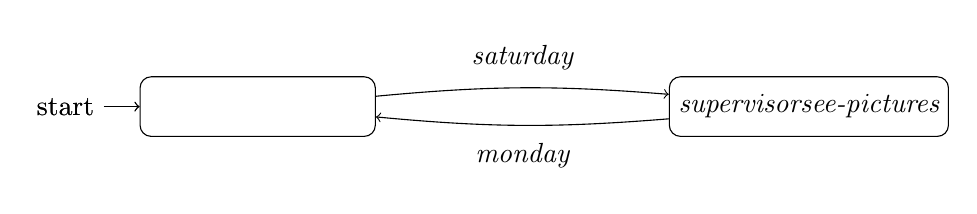
\begin{tikzpicture}[every text node part/.style={align=center},on grid,auto, minimum height=5ex]
      \node (s_0) [initial, initial, rectangle, rounded corners, draw, minimum width=85pt]%
            {~};
      \node (s_1) [rectangle, rounded corners, draw,minimum width=85pt]%
            [right = 7cm of s_0]%
            {$\ff{\textit{supervisor}}{\textit{see-pictures}}$};
            %%{~};
      \path[->] [bend left = 5] (s_1) edge node {$\textit{monday}$} (s_0);
      \path[->] [bend left = 5] (s_0) edge node {$\textit{saturday}$} (s_1);
    \end{tikzpicture}
}}

The automaton is composed by two states. An initial state in which no static policies need to be enforced and another state in which the policy $\ff{\textit{supervisor}}{\textit{see-pictures}}$ is activated. The transitions are labelled with events reported by the social network. The outgoing transition in the initial state is triggered when the social network reports that Saturday started to the automaton. At this moment, the automaton reports to the social network that the policy needs to be activated. Similarly, when Monday starts and it is communicated to the automaton, it updates again its state and the policy is disabled.
\end{example}

Policy automata can be converted to \emph{Dynamic Automata with Timers and Events} (DATEs) \cite{CPS08lrt} which are symbolic automata aimed at representing monitors and have the compilation tool \larva. We implemented the link between \larva~monitors (implementing our policy automata) and the open-source social network Diaspora*~\cite{DiasporaWeb}, thus providing support for some evolving privacy policies~\cite{ppfDiaspora}.
\vspace{-1mm}
\subsection{\tfppf}

\tfppf~stands for {\em Temporal First-Order Privacy Policy Framework}.
It is a formal framework based on epistemic logic~\cite{FHM+95rk} to express and reason about {\em dynamic} and {\em recurrent} privacy policies that are activated or deactivated by context (events) or time. We take \fppf~\cite{PS14fpp} as a point of departure. \fppf~is a formal framework for privacy policies which consists of:
i) A generic social network model (SNM);
ii) A knowledge-based logic (\kbl) to reason about the social network and privacy policies;
iii) A formal language (\ppl) to describe privacy policies (based on the previous logic).
\fppf~is a an expressive privacy policy framework able to represent all privacy policies for social networks like Facebook and Twitter, and beyond~\cite{PS14fpp}. Though rich in what concerns to its expressiveness, \fppf~is not suitable to express evolving privacy policies, in the sense discussed in Section~\ref{sec:motivation}. Therefore, \tfppf~was extended with the following components:

\begin{inparaenum}[]
\item \textbf{Traces of SNMs.} In \fppf~we checked whether a policy is in conformance with an SNM, which is a static picture of the system at a moment in time. For evolving policies it is not enough. We need to consider all the SNMs included in the time-frame in which the policy must hold. Therefore, the satisfaction relation for \tkbl~and the conformance relation for \tppl~both take as a parameter a trace of SNMs. A trace of SNMs is just a sequence of pairs containing an SNM and a timestamp, which indicates the state of the system and the point in time.
  
\item \textbf{Temporal modalities in \tkbl.} The knowledge based logic, \kbl, also needed to be extended. \kbl~is a first order logic which includes the knowledge modality $K$ from epistemic logic. Using the logic we can reason about what the users know, who are their relationships and what they are permitted to do. However, it was not syntactically possible to specify that a given properties always (\al) holds in a trace or eventually will hold (\ev). Moreover, the conformance relation for privacy policies depends on \tkbl's satisfaction relation and as we describe below it requires a certain policy to always hold for a given trace.
  
\item \textbf{Time fields in \tppl.} In \ppl~(the untimed version of the privacy policy language) we were able to express all privacy policies of Facebook and Twitter~\cite{PS14fpp}, and we conjecture that the language is more expressive that the access control protection present in social networks~\cite{BFS+12rbaceehl,F11rbacppl} (though formally showing it is part of our future work). In \tppl, we add a time field where we express the starting time of the privacy policies, i.e., the moment in time from which it is active; the durantion of the policy, for how long will it be activated, for instance, 6 hours, a day, 10 minutes and so on; and the recurrence of the policy, e.g., monthly, daily, yearly, every other day, etc.

\end{inparaenum}

  \begin{example}
  Take as an example the policy we modelled using policy automata ``My supervisor cannot see my pictures during the weekend''. First, let us model the static part of the policy, i.e., ``My supervisor cannot see my pictures''. We can use the untimed \ppl~for it,
  $ \policy{\forall \eta. \neg K_{\mathit{supervisor(me)}} picture(\eta)}{\mathit{me}}$
  where $\eta \in \nat$ is an index for pictures, $\ag$ is the set of all users in the social network, $\mathit{me} \in \ag$ is a user and $\mathit{supervisor} : \ag \rightarrow \ag$ is a function returning the supervisor of a given user. $K_{\mathit{supervisor(me)}} picture(\eta)$ reads as ``My supervisor knows picture($\eta$)'', since the formula is negated we state the desired policy. In order to transform this policy into an evolving one we need to add the temporal part, i.e., ``during the weekend''. \tppl~offers support for it. Assuming that we activate the policy on Saturday 27-08-2016, the policy is written as follows
  $\policy{\forall \eta. \neg K_{\mathit{supervisor(me)}} picture(\eta)}{\mathit{me}}^{[ ~ \text{27-08-2016} ~ \mid ~ \text{2 days} ~ \mid ~ \text{weekly} ~ ]}.$
  Concretly, the format of the time field of \tppl~privacy policies is $[\text{start} $ $\mid $ $\text{duration} \mid \text{recurrence} ]$. Thus, the previous must be enforced from 27-08-2016 (which is Saturday) during 2 days (the weekend) and weekly (every weekend).
    \end{example}

\section{Current and Future Work}

TBW.


\bibliographystyle{abbrv}
\bibliography{references}

\end{document}
